% 2012
% Maciej Szeptuch
% II UWr

\documentclass[11pt,leqno]{article}

\usepackage[utf8]{inputenc}
\usepackage{polski}
\usepackage{a4wide}
\usepackage[cm]{fullpage}

\usepackage{graphicx}
\usepackage{epstopdf}
\usepackage{amsmath,amssymb}
\usepackage{bm}
\usepackage{amsthm}

%% Kropka po numerze paragrafu, podparagrafu, itp.
\makeatletter
    \renewcommand\@seccntformat[1]{\csname the#1\endcsname.\quad}
    \renewcommand\numberline[1]{#1.\hskip0.7em}
\makeatother

%% Numeracja wzorów
\renewcommand{\theequation}{\arabic{section}.\arabic{equation}}

%%%%%%%%%%%%%%%%%%%%%%%%%%%%%%%%%%%%%%%%%%%%%%%%%%%%%%%%%%%%%%%%%%%%%%%%%%%%%%%%

\title{\LARGE \textbf{{Pracownia z analizy numerycznej}}\\
      {\Large Sprawozdanie do zadania \textbf{P1.13.}}\\
      {\large Prowadzący: dr Paweł Woźny}
}
\author{Maciej Szeptuch}
\date{Wrocław, \today}

\begin{document}
\thispagestyle{empty}
\maketitle

%%%%% WSTĘP
\section{Wstęp - Równania rekurencyjne}\label{S:Wstęp}
Najprostsze równania rekurencyjne poznaliśmy już w szkole w postaci np. ciągu arytmetycznego, czy geometrycznego.
W późniejszym okresie naszej edukacji zetknęliśmy się też np. z ciągiem Fibonacciego.
Ciągi tego typu(\textit{zdefiniowane rekurencyjnie}) mają szerokie zastosowanie nie tylko w teorii matematycznej ale także w innych dziedzinach.
Używa się ich w biologii - przy modelowaniu wzrostu populacji, interakcji pomiędzy populacjami,
ekonomii - do modelowania zmian na rynkach itp.,
czy elektronice - w przetwarzaniu sygnałów cyfrowych.
Mimo tego, że z pozoru wydają się nieskomplikowane, równania te potrafią sprawiać wiele problemów -
od czysto wydajnościowych, liczenie $n$-tego wyrazu ciągu z definicji potrafi chwilę trwać,
do problemów z dokładnością, gdy np. liczymy $n$-ty wyraz ciągu Fibonacciego za pomocą wzoru ogólnego tzw. wzoru Bineta,
gdzie przy stosunkowo niewielkich błędach zaokrągleń możemy minąć się z poprawnym wynikiem o kilka jednostek.
Tego typu równanie występuje w rozważanym przeze mnie problemie. Dokładniej zajmowałem się ciągiem:
\begin{equation}\label{E:Ciąg}
    I_{n} = \int_{0}^{1} \frac{x^n}{x+10} \mathrm{d}x
\end{equation}
Który po odpowiednich przekształceniach(patrz \ref{S:Dowody} Dowody) można reprezentować w postaci równania rekurencyjnego:
\begin{equation}\label{E:Rekurencja}
    I_{n} + 10I_{n-1} = \frac{1}{n}\qquad \mbox{(dla $n \geq 0$, $I_{0} = \log{\frac{11}{10}}$)}
\end{equation}
\section{Dowody}\label{S:Dowody}
Częścią zadania jest wykazanie trzech następujących własności:
\subsection{Dowód 1}\label{SS:Dowód 1}
$$
    I_{0} = \log\frac{11}{10}
$$
Korzystając bezpośrednio z definicji \eqref{E:Ciąg} wyliczamy $I_{0}$:
$$
    I_{0} =
    \int_{0}^{1} \frac{x^0}{x+10} \mathrm{d}x =
    \int_{0}^{1} \frac{1}{x+10} \mathrm{d}x =
    \log|x+10| \Bigg|_{0}^{1} =
    \log(11) - \log(10) =
    \log\frac{11}{10}
$$
\subsection{Dowód 2}\label{SS:Dowód 2}
$$
    I_{n} + 10I_{n-1} = \frac{1}{n}
$$
Również korzystając z definicji \eqref{E:Ciąg} rozpisujemy $I_{n}$ oraz $I_{n-1}$:
$$
    I_{n} + 10I_{n-1} =
    \int_{0}^{1} \frac{x^n}{x+10} \mathrm{d}x + 10\int_{0}^{1} \frac{x^{n-1}}{x+10} \mathrm{d}x =
$$
następnie możemy połączyć te całki w jedną(takie same granice całkowania):
$$
    =
    \int_{0}^{1} \frac{x^n + 10x^{n-1}}{x+10} \mathrm{d}x =
$$
wyciągamy $x^{n-1}$ przed ułamek:
$$
    =
    \int_{0}^{1} x^{n-1}\frac{x + 10}{x + 10} \mathrm{d}x =
    \int_{0}^{1} x^{n-1} \mathrm{d}x =
$$
i otrzymujemy ostateczny wynik:
$$
    =
    \frac{x^n}{n} \Bigg|_{0}^{1} =
    \frac{1}{n}
$$
\subsection{Dowód 3}\label{SS:Dowód 3}
$$
    \frac{1}{11(n+1)} \leq I_{n} \leq \frac{1}{10(n+1)}
$$
Najpierw zajmiemy się pierwszą nierównością $\frac{1}{11(n+1)} \leq I_{n}$. Korzystamy z definicji ciągu \eqref{E:Ciąg}:
$$
    I_{n} =
    \int_{0}^{1} \frac{x^n}{x+10} \mathrm{d}x =
$$
Wyciągamy $x^n$ przed ułamek i korzystamy z całkowania przez części:
$$
    =
    \int_{0}^{1} x^n\frac{1}{x+10} \mathrm{d}x =
    \int_{0}^{1} \Bigg(\frac{x^{n+1}}{n+1}\Bigg)' \frac{1}{x+10} \mathrm{d}x =
$$
$$
    =
    \frac{x^{n+1}}{n+1}\frac{1}{x+10} \Bigg|_{0}^{1} + \int_{0}^{1} \frac{x^{n+1}}{n+1} \frac{1}{(x+10)^2} \mathrm{d}x =
$$
$$
    =
    \frac{1}{11(n+1)} + \int_{0}^{1} \frac{x^{n+1}}{(n+1)(x+10)^2} \mathrm{d}x
$$
Możemy zauważyć, że $\int_{0}^{1} \frac{x^{n+1}}{(n+1)(x+10)^2} \mathrm{d}x$ jest zawsze nieujemna(funkcja
podcałkowa ma wartości nieujemne na przedziale [0,1]), więc możemy oszacować wartość $I_{n}$ od dołu
pozbywając się tego dodatniego czynnika. \\ W efekcie otrzymujemy:
$$
    \frac{1}{11(n+1)} \leq I_{n}
$$ \\
Teraz czas na drugą nierówność $I_{n} \leq \frac{1}{10(n+1)}$.
Tak jak w poprzednim przypadku całkujemy przez części, tylko tym razem robimy to jeden raz więcej:
$$
    I_{n} =
    \frac{1}{11(n+1)} + \int_{0}^{1} \frac{x^{n+1}}{(n+1)(x+10)^2} \mathrm{d}x =
$$
$$
    =
    \frac{1}{11(n+1)} + \int_{0}^{1} \frac{x^{n+1}}{n+1}\frac{1}{(x+10)^2} \mathrm{d}x =
$$
$$
    =
    \frac{1}{11(n+1)} + \int_{0}^{1} \Bigg(\frac{x^{n+2}}{(n+1)(n+2)}\Bigg)'\frac{1}{(x+10)^2} \mathrm{d}x =
$$
$$
    =
    \frac{1}{11(n+1)} + \Bigg(\frac{x^{n+2}}{(n+1)(n+2)}\frac{1}{(x+10)^2}\Bigg|_{0}^{1} - 2\int_{0}^{1} \frac{x^{n+2}}{(n+1)(n+2)}\frac{1}{(x+10)^3} \mathrm{d}x =
$$
$$
    =
    \frac{1}{11(n+1)} + \frac{1}{11^2(n+1)(n+2)} - 2\int_{0}^{1} \frac{x^{n+2}}{(n+1)(n+2)}\frac{1}{(x+10)^3} \mathrm{d}x =
$$
$$
    =
    \frac{1}{11(n+1)}\Bigg(1 + \frac{1}{11(n+2)}\Bigg) - 2\int_{0}^{1} \frac{x^{n+2}}{(n+1)(n+2)}\frac{1}{(x+10)^3} \mathrm{d}x
$$
Całka(tak jak poprzednio) przyjmuje wartości dodatnie czyli w połączeniu z $-2$ zawsze zmniejsza nam wartość $I_{n}$,
więc przy szacowaniu z góry możemy ją pominąć.
Zostaje nam teraz tylko $\frac{1}{11(n+1)}\Big(1 + \frac{1}{11(n+2)}\Big)$, które możemy oszacować z góry przez:
$$
    \frac{1}{11(n+1)}\Bigg(1 + \frac{1}{11(n+2)}\Bigg) \leq \frac{1}{10(n+1)}
$$
Ponieważ możemy to pomnożyć stronami przez $10\cdot11(n+1)$ i uzyskamy
$$
    10 + \frac{10}{11(n+2)} \leq 11
$$
a w efekcie
$$
    \frac{10}{11(n+2)} \leq 1
$$
co jest oczywiste dla $n \in \mathbb{N}$.
Doprowadziło nas to do szukanej nierówności:
$$
    I_{n} \leq \frac{1}{10(n+1)}
$$
\section{Doświadczenie}\label{S:Doświadczenie}
Korzystając z równania rekurencyjnego \eqref{E:Rekurencja} wyliczono 20 początkowych wyrazów ciągu,
najpierw w kolejności rosnącej od $I_{0} = \log\frac{11}{10}$, a następnie malejącej przy założeniu,
że $I_{21} = 0$. Do obliczeń wykorzystano program w C++\footnote{program.cpp w katalogu prog},
używając float i double dla odpowiednio obliczeń pojedynczej i podwójnej precyzji.
Wartości dokładne zostały uzyskane przy pomocy Wolframa\footnote{https://www.wolframalpha.com/}.
\subsection{Obliczenia w kierunku rosnącego n}\label{SS:Rosnaco}
\begin{table}[!h]
\renewcommand{\arraystretch}{1.1}
\vspace{-2em}
\caption{Wartości $I_{n}$ licząc od 0 do 20 przy pomocy równania rekurencyjnego \eqref{E:Rekurencja}}\label{T:RekurencjaDoPrzodu}
\vspace{-1em}
\begin{center}
    \begin{tabular}{r|r|r|l}
        \texttt{$i$}  &       \texttt{float}      &           \texttt{double}         &    \texttt{Wolfram}   \\ \hline
        $0$           &  $\underline{0.095310}20$ & $\underline{0.095310179804324}93$ & $0.09531017980432486$ \\
        $1$           &  $\underline{0.04689}795$ & $\underline{0.04689820195675}065$ & $0.04689820195675139$ \\
        $2$           &  $\underline{0.0310}2052$ & $\underline{0.0310179804324}9349$ & $0.03101798043248600$ \\
        $3$           &  $\underline{0.0231}2812$ & $\underline{0.023153529008}39845$ & $0.02315352900847328$ \\
        $4$           &  $\underline{0.018}71878$ & $\underline{0.01846470991}601545$ & $0.01846470991526710$ \\
        $5$           &  $\underline{0.01}281221$ & $\underline{0.0153529008}3984547$ & $0.01535290084732893$ \\
        $6$           &  $\underline{0.0}3854455$ & $\underline{0.013137658}26821192$ & $0.01313765819337728$ \\
        $7$           &            $-0.24258836$  & $\underline{0.011480560}17502364$ & $0.01148056092337000$ \\
        $8$           &             $2.55088353$  & $\underline{0.01019439}824976365$ & $0.01019439076629997$ \\
        $9$           &           $-25.39772415$  & $\underline{0.009167}12861347463$ & $0.00916720344811136$ \\
        $10$          &           $254.07723999$  & $\underline{0.00832}871386525372$ & $0.00832796551888631$ \\
        $11$          &         $-2540.68164062$  & $\underline{0.00762}195225655374$ & $0.00762943572022778$ \\
        $12$          &         $25406.90039062$  & $\underline{0.007}11381076779595$ & $0.00703897613105545$ \\
        $13$          &       $-254068.92187500$  & $\underline{0.00}578496924511744$ & $0.00653331561252232$ \\
        $14$          &       $2540689.25000000$  & $\underline{0.0}1357887897739715$ & $0.00609541530334816$ \\
        $15$          &     $-25406892.00000000$  &           $-0.06912212310730485$  & $0.00571251363318499$ \\
        $16$          &     $254068928.00000000$  & $\underline{0.}75372123107304856$ & $0.00537486366815008$ \\
        $17$          &   $-2540689408.00000000$  &           $-7.47838878131872065$  & $0.00507489273026384$ \\
        $18$          &   $25406894080.00000000$  &           $74.83944336874276360$  & $0.00480662825291712$ \\
        $19$          & $-254068948992.00000000$  &         $-748.34180210848023762$  & $0.00456529641819718$ \\
        $20$          & $2540689424384.00000000$  &         $7483.46802108480278548$  & $0.00434703581802810$ \\
    \end{tabular}
\end{center}
\vspace{-1,5em}
\end{table}
Na podstawie Tabeli \ref{T:RekurencjaDoPrzodu} możemy zauważyć, że w (\textit{prawie}) każdym kroku maleje nam
dokładność o jedną cyfrę dziesiętną i odpowiednio dla liczb o pojedynczej i podwójnej precyzji od $n = 7$
bądź $n = 15$ wyniki są już praktycznie bezwartościowe. Głównym powodem tego, że w przypadku typu double sensowne
wyniki otrzymujemy dla większej liczby elementów jest zwyczajnie to, że początkowe przybliżenie zostało zapamiętane dokładniej.
Bez względu na dokładność arytmetyki tracimy jedną cyfrę dokładności na (\textit{prawie}) każdą iteracje.
Dlaczego tak jest? Aby odpowiedzieć na to pytanie musimy przyjrzeć się dokładniej danej rekurencji \eqref{E:Rekurencja}.
$$
    I_{n} + 10I_{n-1} = \frac{1}{n}
$$
Już na pierwszy rzut oka możemy przypuszczać, że ma to związek z $10$ przy $I_{n-1}$ - jakikolwiek błąd miał
ten element zostanie tutaj powiększony o $10$ i z jego pomocą będziemy starali się wyliczyć następny element ciągu.
Ale spróbujmy pokazać to trochę formalniej. \\
Dla ustalenia uwagi $M_{n}$ - nazwę elementy naszego ciągu wyliczane przez program, a oryginalne $I_{n}$ -
będą dokładnymi wynikami jakie powinniśmy uzyskiwać. Z tego, że obliczenia na komputerze nie są dokładne wynika:
\begin{equation}\label{E:CiągNaKomputerze}
    M_{n} = I_{n} + e_{n}\qquad\mbox{(gdzie $e_{n}$ to błąd bezwzględny wyliczenia)}
\end{equation}
Teraz liczymy kolejne elementy:
$$
    M_{n} + 10M_{n-1} = \frac{1}{n}
$$
Jak rozpiszemy $M_{n}$ z \eqref{E:CiągNaKomputerze} dostaniemy:
$$
    I_{n} + 10I_{n-1} + e_{n} + 10e_{n-1} = \frac{1}{n}
$$
Ale zakładamy, że dla dokładnych wartości zachodzi:
$$
    I_{n} + 10I_{n-1} = \frac{1}{n}
$$
Dzięki czemu otrzymujemy:
$$
    e_{n} = -10e_{n-1}
$$
Z którego wynika, że:
$$
    \frac{|e_{n}|}{|e_{n-1}|} = 10
$$
Czyli tak jak przypuszczaliśmy błąd kolejnego elementu jest 10 razy większy niż poprzedniego,
co także ilustruje Rysunek \ref{G:WykresBleduDoPrzodu}.
\begin{center}
    \begin{figure}[!h]
        \vspace{-2em}
        \begin{center}
        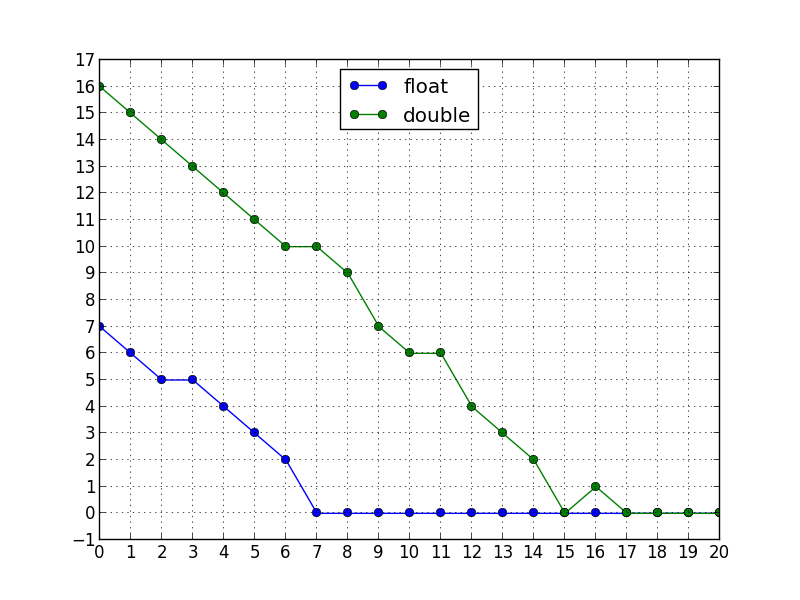
\includegraphics[scale=0.5,angle=0]{wykresbledudoprzodu.png}
        \vspace{-2,5em}
        \caption{Liczba cyfr dokładnych przy obliczaniu \eqref{E:Rekurencja} od $n=0$ do $n=20$}\label{G:WykresBleduDoPrzodu}
    \end{center}
    \vspace{-2em}
    \end{figure}
\end{center}
\subsection{Obliczenia w kierunku malejącego n}\label{SS:Malejaco}
W tym zadaniu założyliśmy że $I_{21} = 0$, dlaczego jest to sensowne przybliżenie? Zapewne dlatego,
że błąd bezwzględny jest zaledwie rzędu $10^{-3}$. Dokładna wartość $I_{21}$ wynosi około $0.00414868$. \\
\begin{table}[!h]
\renewcommand{\arraystretch}{1.1}
\caption{Wartości $I_{n}$ licząc od 20 do 0 przy pomocy równania rekurencyjnego \eqref{E:Rekurencja}}\label{T:RekurencjaWstecz}
\vspace{-1em}
\begin{center}
    \begin{tabular}{r|l|l|l}
        \texttt{$i$}  &         \texttt{float}      &          \texttt{double}            &    \texttt{Wolfram}     \\ \hline
        $20$          & $\underline{0.004}76190494$ & $\underline{0.004}7619047619047614$ & $0.0043470358180281090$ \\
        $19$          & $\underline{0.0045}2380953$ & $\underline{0.0045}238095238095245$ & $0.0045652964181971890$ \\
        $18$          & $\underline{0.0048}1077703$ & $\underline{0.0048}107769423558887$ & $0.0048066282529171231$ \\
        $17$          & $\underline{0.005074}47775$ & $\underline{0.005074}4778613199658$ & $0.0050748927302638432$ \\
        $16$          & $\underline{0.005374}90519$ & $\underline{0.005374}9051550444739$ & $0.0053748636681500862$ \\
        $15$          & $\underline{0.0057125}0962$ & $\underline{0.0057125}094844955523$ & $0.0057125136331849913$ \\
        $14$          & $\underline{0.006095415}91$ & $\underline{0.006095415}7182171115$ & $0.0060954153033481675$ \\
        $13$          & $\underline{0.006533315}87$ & $\underline{0.006533315}5710354303$ & $0.0065333156125223261$ \\
        $12$          & $\underline{0.007038976}07$ & $\underline{0.00703897613}52041505$ & $0.0070389761310554596$ \\
        $11$          & $\underline{0.00762943}644$ & $\underline{0.0076294357}198129171$ & $0.0076294357202277873$ \\
        $10$          & $\underline{0.008327965}62$ & $\underline{0.008327965518}9277997$ & $0.0083279655188863121$ \\
        $9$           & $\underline{0.009167203}68$ & $\underline{0.0091672034481}072202$ & $0.0091672034481113687$ \\
        $8$           & $\underline{0.01019439}101$ & $\underline{0.010194390766}3003888$ & $0.0101943907662999742$ \\
        $7$           & $\underline{0.011480560}53$ & $\underline{0.0114805609233}699611$ & $0.0114805609233700025$ \\
        $6$           & $\underline{0.01313765}906$ & $\underline{0.01313765819337728}81$ & $0.0131376581933772854$ \\
        $5$           & $\underline{0.01535290}209$ & $\underline{0.01535290084732893}71$ & $0.0153529008473289381$ \\
        $4$           & $\underline{0.0184647}1056$ & $\underline{0.01846470991526710}79$ & $0.0184647099152671061$ \\
        $3$           & $\underline{0.02315352}857$ & $\underline{0.0231535290084732}906$ & $0.0231535290084732893$ \\
        $2$           & $\underline{0.03101798}333$ & $\underline{0.03101798043248600}24$ & $0.0310179804324860043$ \\
        $1$           & $\underline{0.046898201}11$ & $\underline{0.046898201956751}4008$ & $0.0468982019567513995$ \\
        $0$           & $\underline{0.0953101}8138$ & $\underline{0.0953101798043248}519$ & $0.0953101798043248600$ \\
    \end{tabular}
\end{center}
\vspace{-1,5em}
\end{table}
Na podstawie Tabeli \ref{T:RekurencjaWstecz} już na pierwszy rzut oka widać różnicę i poprawę - wyniki nie rozbiegają się do nieskończoności.
Ponadto możemy zauważyć, że ulegają poprawie z (\textit{prawie}) każdym krokiem o jedną cyfrę dziesiętną, dzięki czemu są dokładniejsze niż w przypadku poprzedniego zastosowania rekurencji.
Przeprowadzając bardzo podobne rozumowanie jak wcześniej możemy dojść do wyniku:
$$
    \frac{|e_{n-1}|}{|e_{n}|} = \frac{1}{10}
$$
Który potwierdza, że z każdym krokiem błąd maleje dziesięciokrotnie, aż do osiągnięcia dokładności arytmetyki po czym stabilizuje się w jej okolicach.
Ilustruje to Rysunek \ref{G:WykresBleduWstecz}.
\begin{center}
    \begin{figure}[!h]
        \vspace{-2em}
        \begin{center}
        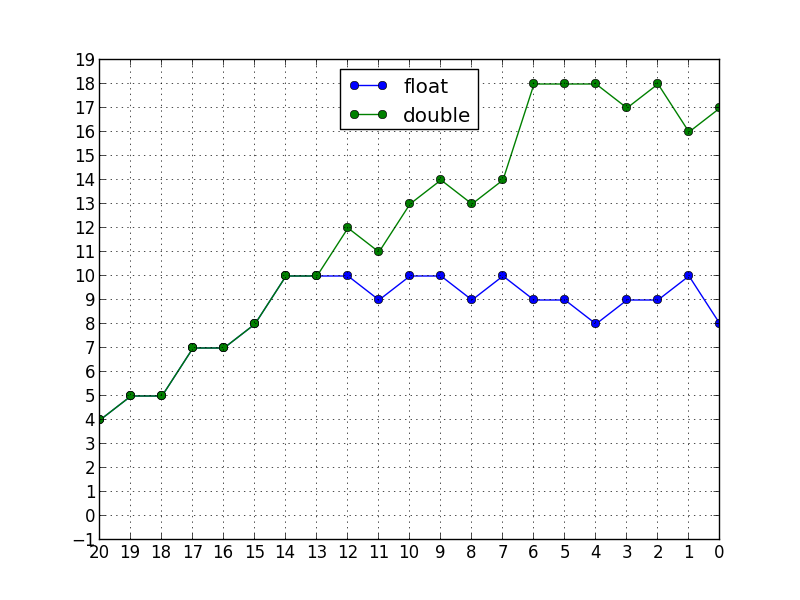
\includegraphics[scale=0.5,angle=0]{wykresbleduwstecz.png}
        \vspace{-2,5em}
        \caption{Liczba cyfr dokładnych przy obliczaniu \eqref{E:Rekurencja} od $n=20$ do $n=0$}\label{G:WykresBleduWstecz}
    \end{center}
    \vspace{-2em}
    \end{figure}
\end{center}
\section{Końcowe wnioski}\label{S:Wnioski}
Jak możemy zauważyć na podstawie przeprowadzonych doświadczeń, równania rekurencyjne nie są wcale takie nieskomplikowane jak mogłoby się wydawać.
W przypadku obliczeń na komputerach, gdzie nie możemy reprezentować danych dokładnie, bardzo ważne znaczenie mają własności takiego równania.
Jak w tym przypadku właśnie propagacja błędu w przypadku użycia tej rekurencji wprost, a znaczne polepszenie wyników poprzez niedokładne założenie co do
wartości dalszego elementu i wyliczanie szukanych wstecz. Ta technika była już znana od dawna.
Już koło 1952 r. Dr. J. C. P. Miller\footnote{http://en.wikipedia.org/wiki/J.\_C.\_P.\_Miller} wykorzystał tę metodę, własność do wyliczania kolejnych funkcji Bessela pierwszego rodzaju($J_\alpha(x)$, dla całkowitych $\alpha$), które są rozwiązaniami tzw.
równania Bessela\footnote{http://en.wikipedia.org/wiki/Bessel\_function}
$$
    x^{2} \frac{d^{2} y}{dx^{2}} + x \frac{dy}{dx} + (x^{2} - \alpha^{2})y = 0
$$
równania różniczkowego drugiego stopnia używanego między innymi w analizie fal elektromagnetycznych, przepływie ciepła itp. Było to możliwe ponieważ spełniają one równanie rekurencyjne:
$$
    \frac{2\alpha}{x} J_\alpha(x) = J_{\alpha-1}(x) + J_{\alpha+1}(x)
$$
które, podobnie jak to rozważane przeze mnie, zaczyna dawać niedokładne wyniki w przypadku obliczania w kolejności rosnącej, a polepsza się przy liczeniu wstecz.
\thispagestyle{empty}
\begin{thebibliography}{99}
    \bibitem{L} S. Lewanowicz, \textit{Notatki do wykładu z analizy numerycznej}, Wrocław, 2012r.
    \bibitem{Wolfram} WolframAlpha, https://www.wolframalpha.com.
    \bibitem{Wikipedia} Wikipedia, https://en.wikipedia.org/wiki/Recurrence\_relation, https://en.wikipedia.org/wiki/Bessel\_function
    \bibitem{M} Thomas E. Michels, \textit{The backward recurrence method for computing regular bessel function}, Washington D.C., 1964r.
\end{thebibliography}
\end{document}
